\begin{frame}{Целесообразность}
    \begin{columns}[T,onlytextwidth]
        \begin{column}{0.56\textwidth}
            \begin{itemize}
                \item<1-> Целесообразность --- предназначенность для определенной цели
                \item<2-> Красота заключалась в простоте и рациональности реализации
                \item<3-> <<Дом-машина для жилья>>
                \item<4-> Содержит всю необходимую инфраструктуру
                \item<5-> Максимально удобная эксплуатация здания
            \end{itemize}
        \end{column}
        \begin{column}{0.5\textwidth}
            \visible<2->{
                \begin{figure}
                    \centering
                    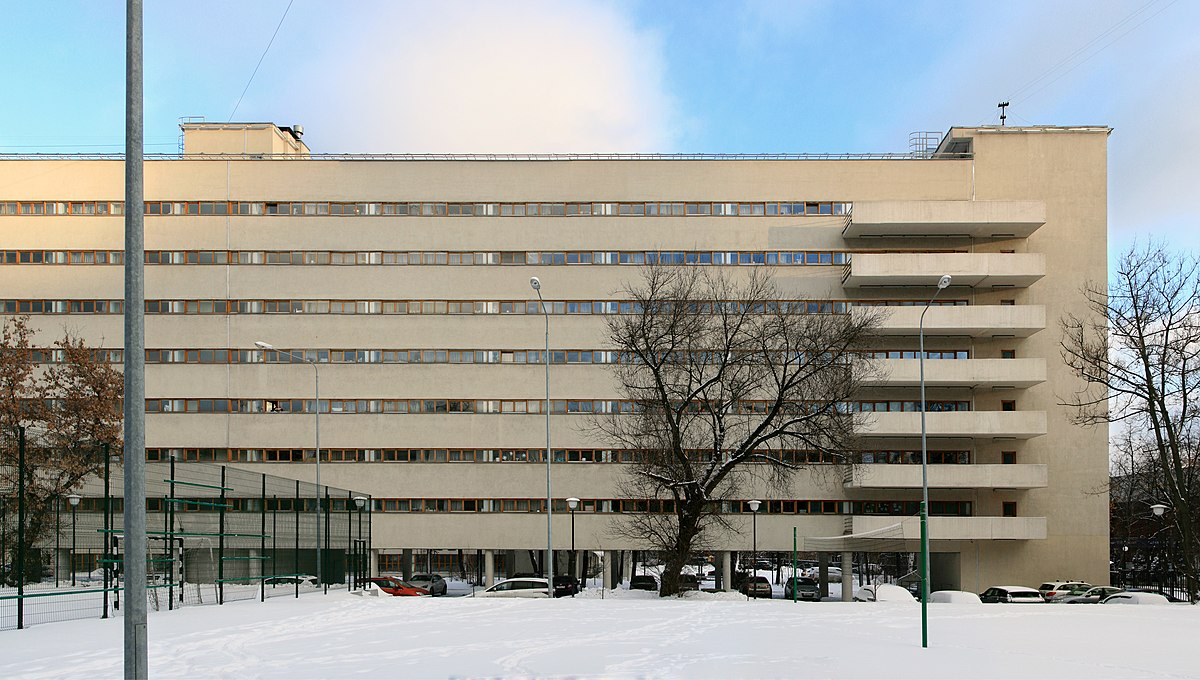
\includegraphics[width=0.9\textwidth]{images/Moscow_Ordzhonikidze8_Y18.jpg}
                    \caption*{Дом-коммуна на ул. Орджоникидзе}
                \end{figure}
            }
        \end{column}
    \end{columns}
\end{frame}